\documentclass{beamer}

\usetheme{default} % You can change the theme as needed
\usepackage{array}

\title{Presentation Title}
\author{Samy Braik}
\date{\today}

\begin{document}

\begin{frame}
    \titlepage
\end{frame}

\begin{frame}{Outline}
    \tableofcontents
\end{frame}

\section{Introduction}

\begin{frame}
    We denote by \(p\) the target distribution and \(q\) an easy-to-sample distribution, for example a centered Gaussian.
\end{frame}

\begin{frame}{Diffusion}
    Let \(X_0\sim p\). We want to add noise until we reach pure noise, and denoise it afterward. We choose an horizon of time \(T\in\mathbb{N}^*\) and a noise schedule \(\beta:[0,T]\rightarrow\mathbb{R}^*\), continuous and non decreasing.

    \begin{block}{Forward process}
            \[d\overrightarrow{X}_t = \frac{-\beta(t)}{2\sigma^2}\overrightarrow{X}_t dt + \sqrt{\beta(t)}dB_t, \quad \overrightarrow{X}_0\sim p\]
    \end{block}

    \begin{block}{Backward process}
        \begin{align*}
            d\overleftarrow{X}_t=&\left(  \frac{\beta(T-t)}{2\sigma^2}\overleftarrow{X}_t+\beta(T-t)\nabla\log p_{T-t}\left(\overleftarrow{X}_t \right)  \right)dt \\ &+ \sqrt{\beta(T-t)}dB_t, \quad \overleftarrow{X}_0\sim p_T
        \end{align*}
            
    \end{block}
\end{frame}

\begin{frame}
    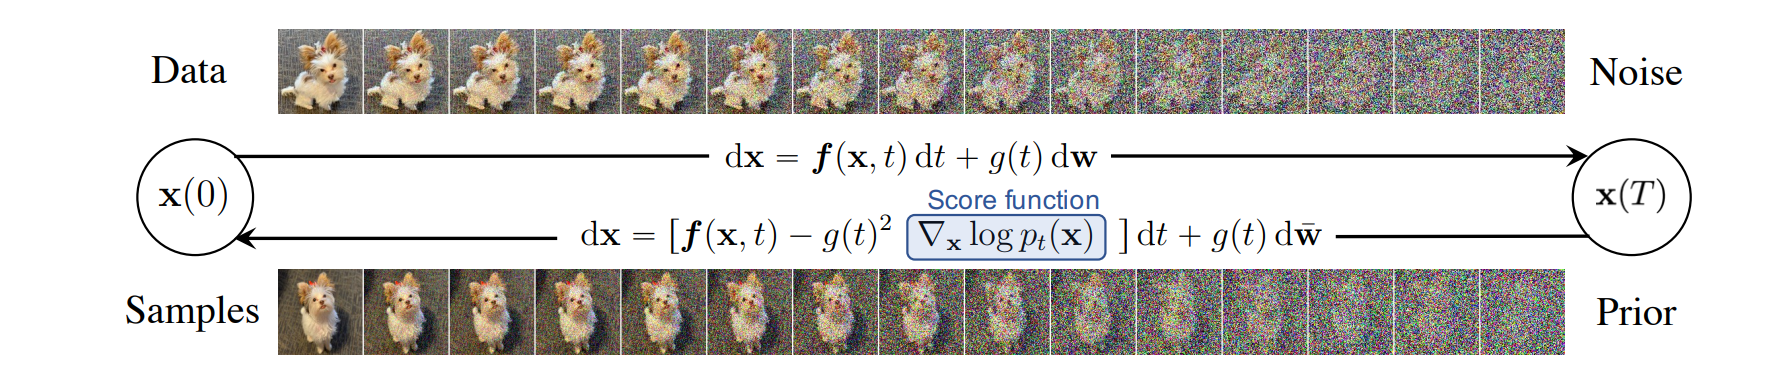
\includegraphics[width=1\linewidth]{score_based_dog.png}
    \bigskip

    We learn the score by using score-matching techniques
    \begin{block}{Score matching}
        \[\mathcal{L}_\text{score}(\theta)=\mathbb{E}\left[ \left\| s_\theta \left(\tau,\overrightarrow{X}_\tau \right)-\log p_\tau \left(\overrightarrow{X}_\tau|X_0 \right)\right\|^2  \right]   \]
    \end{block}
    Plug it in the backward process and generate by discretizing the dynamics.
\end{frame}

\begin{frame}{Normalizing flow}
    Let \(X_0\sim q\) and \(X_1\sim p\). We want to learn \(f_\theta\) such that \(X_1 \simeq f_\theta^(X_0)=Z\sim p_Z\). To do that, we set a structure on \(f_\theta\), with \(f_1,\ldots,f_k\) simpler function (all parametrized by \(\theta\)) such that 
    \[f_\theta=f_1\circ f_2\circ\ldots\circ f_k\] 
    We determine \(f_\theta\) by minimizing 
    \[\mathcal{L}_\text{NF}(\theta)= \mathbb{E}\left[-\log p_Z(f_\theta(x))-\log \left|\det \frac{\partial f_\theta}{\partial x}(x)\right|\right]\]
\end{frame}

\begin{frame}
    A flow is 
\end{frame}

\begin{frame}{Flow matching}
    
\end{frame}



\begin{frame}{Comparison}
    \begin{tabular}{|l|c|r|}
        \hline
        Models & Pros & Cons \\
        \hline
        Diffusion & 1.2 &  \\
        Normalizing flow & Exact density estimation & Computationaly intensive \\ 
        Flow matching & Exact density estimation / SImulation free training  & rzreeq\\
        \hline
      \end{tabular}
    \end{frame}



\end{document}